\section{Auswertung}
\label{sec:Auswertung}

\subsection{Bestimmung von \(R_1\)}
\begin{figure}
  %Plot der Messwerte aus a)
  \centering
  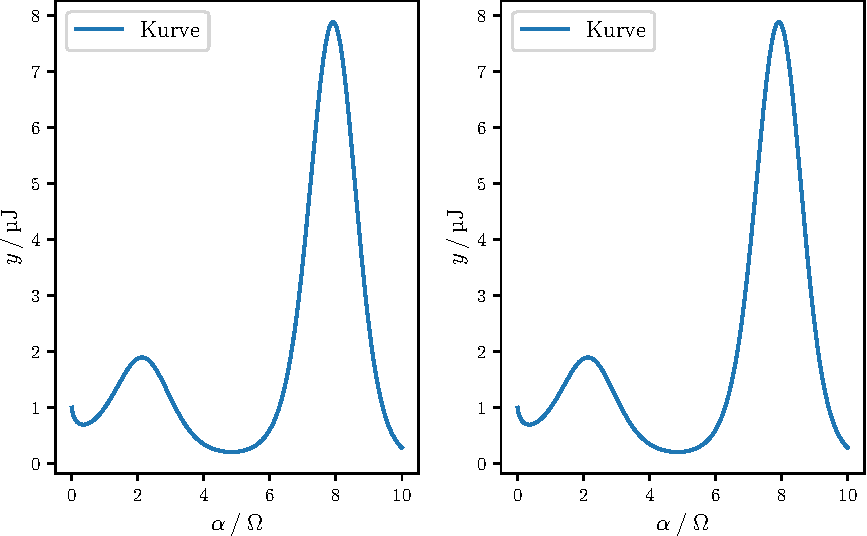
\includegraphics{plot.pdf}
  \caption{Plot.}
  \label{fig:plot}
\end{figure}
Der grüne Vergleichsgraph ist die rechnerisch korrekte Einhüllende mit den gegebenen Werten für Schaltkreis 3.
\begin{table}[htp]
  %Messwerte aus a)
  \centering
  \caption{Tabelle der Messwerte mit \(R_1\).}
  \label{tab:tab1}
  \begin{tabular}{c c}
    \toprule
    U in $V$ & t in $\mu$s\\
    \midrule
    0.2 & 0\\
    0.14 & 25\\
    0.1 & 54\\
    0.07 & 78\\
    0.05 & 105\\
    0.04 & 130\\
    0.03 & 158\\
    0.02 & 184\\
    0.014 & 210\\
    0.008 & 247\\
    \bottomrule
  \end{tabular}
\end{table}
\\
Die Messwerte entsprechen leider nicht der Formel aus dem Versuch, sondern haben starke Abweichungen.

\newpage
\subsection{Bestimmung von \(R_{ap}\)}
Der aperiodische Grenzfall wurde bei einer Signalfrequenz von 1.6\(kHz\) gemessen.\\
Die \autoref{fig:aper} zeigt, dass bei der Einstellung 2.26 am Drehrad(siehe \autoref{fig:drehohm}), sich der aperiodische Grenzfall einstellt.\\
\begin{figure}
  \centering
  \begin{subfigure}{0.9\textwidth}
    \centering
    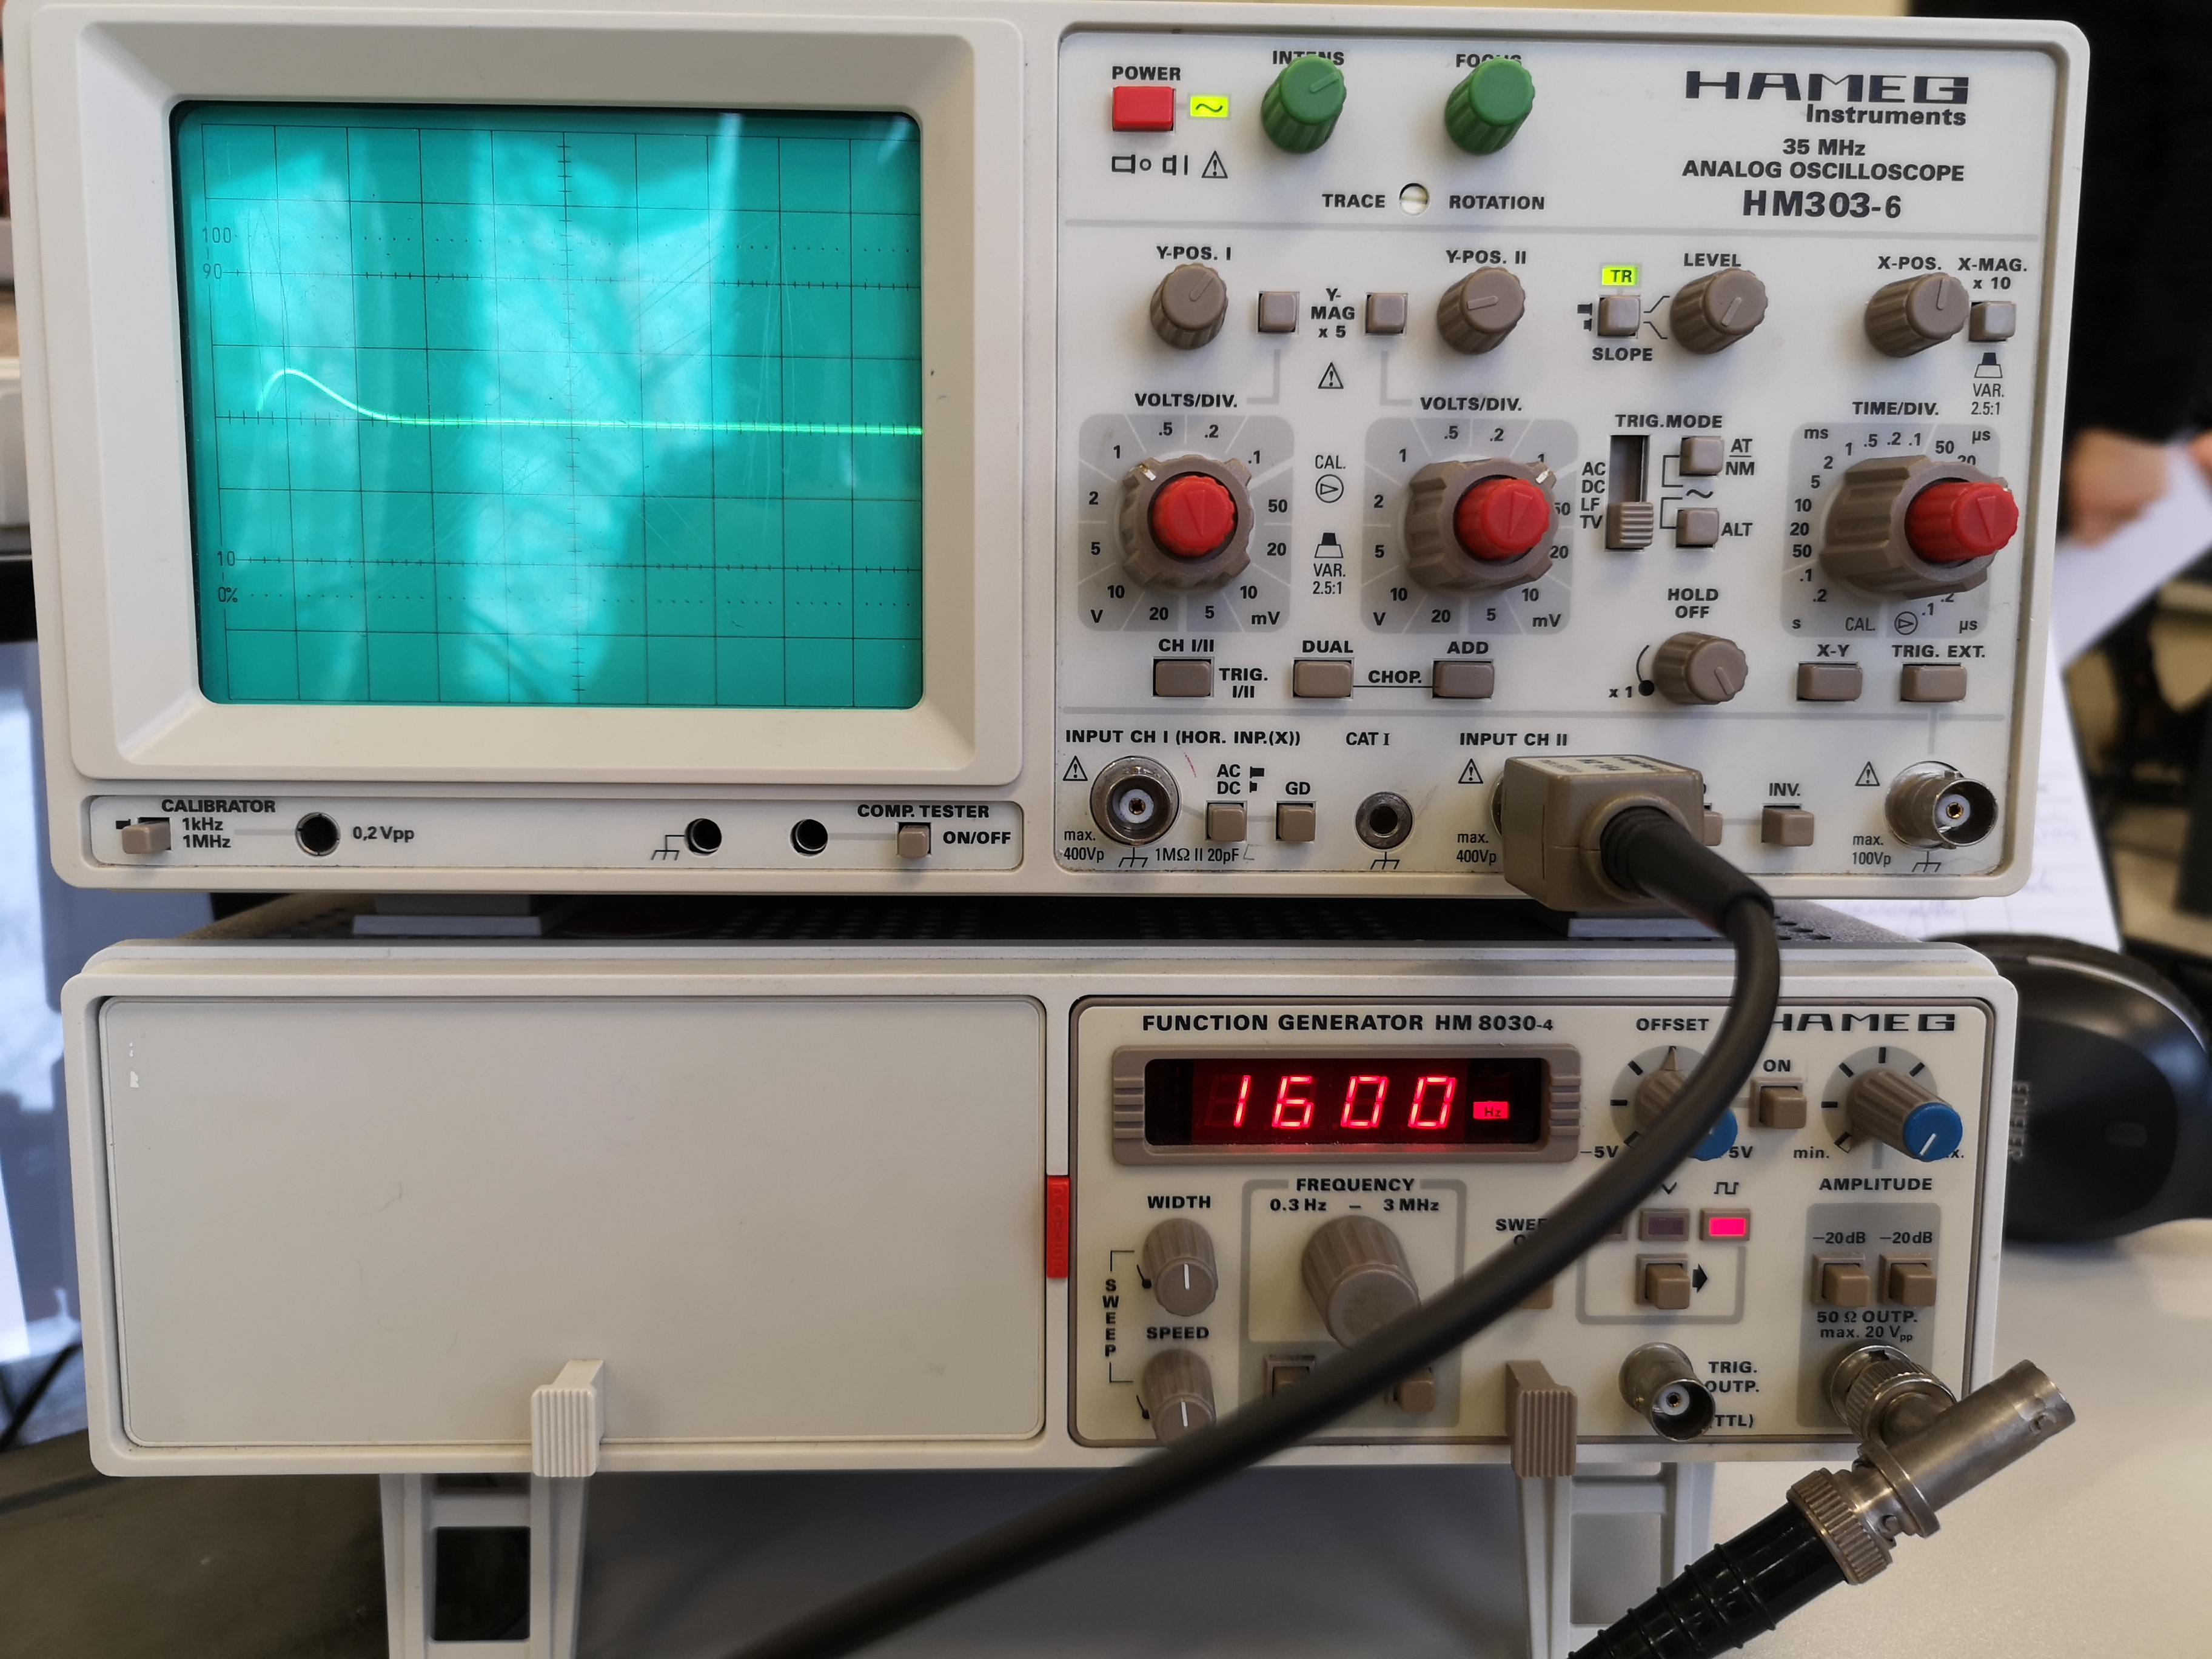
\includegraphics[height=6cm]{content/aperiode.jpg}
    \caption{Aperiodischer Grenzfall.}
    \label{fig:aper}
  \end{subfigure}
  \begin{subfigure}{0.9\textwidth}
    \centering
    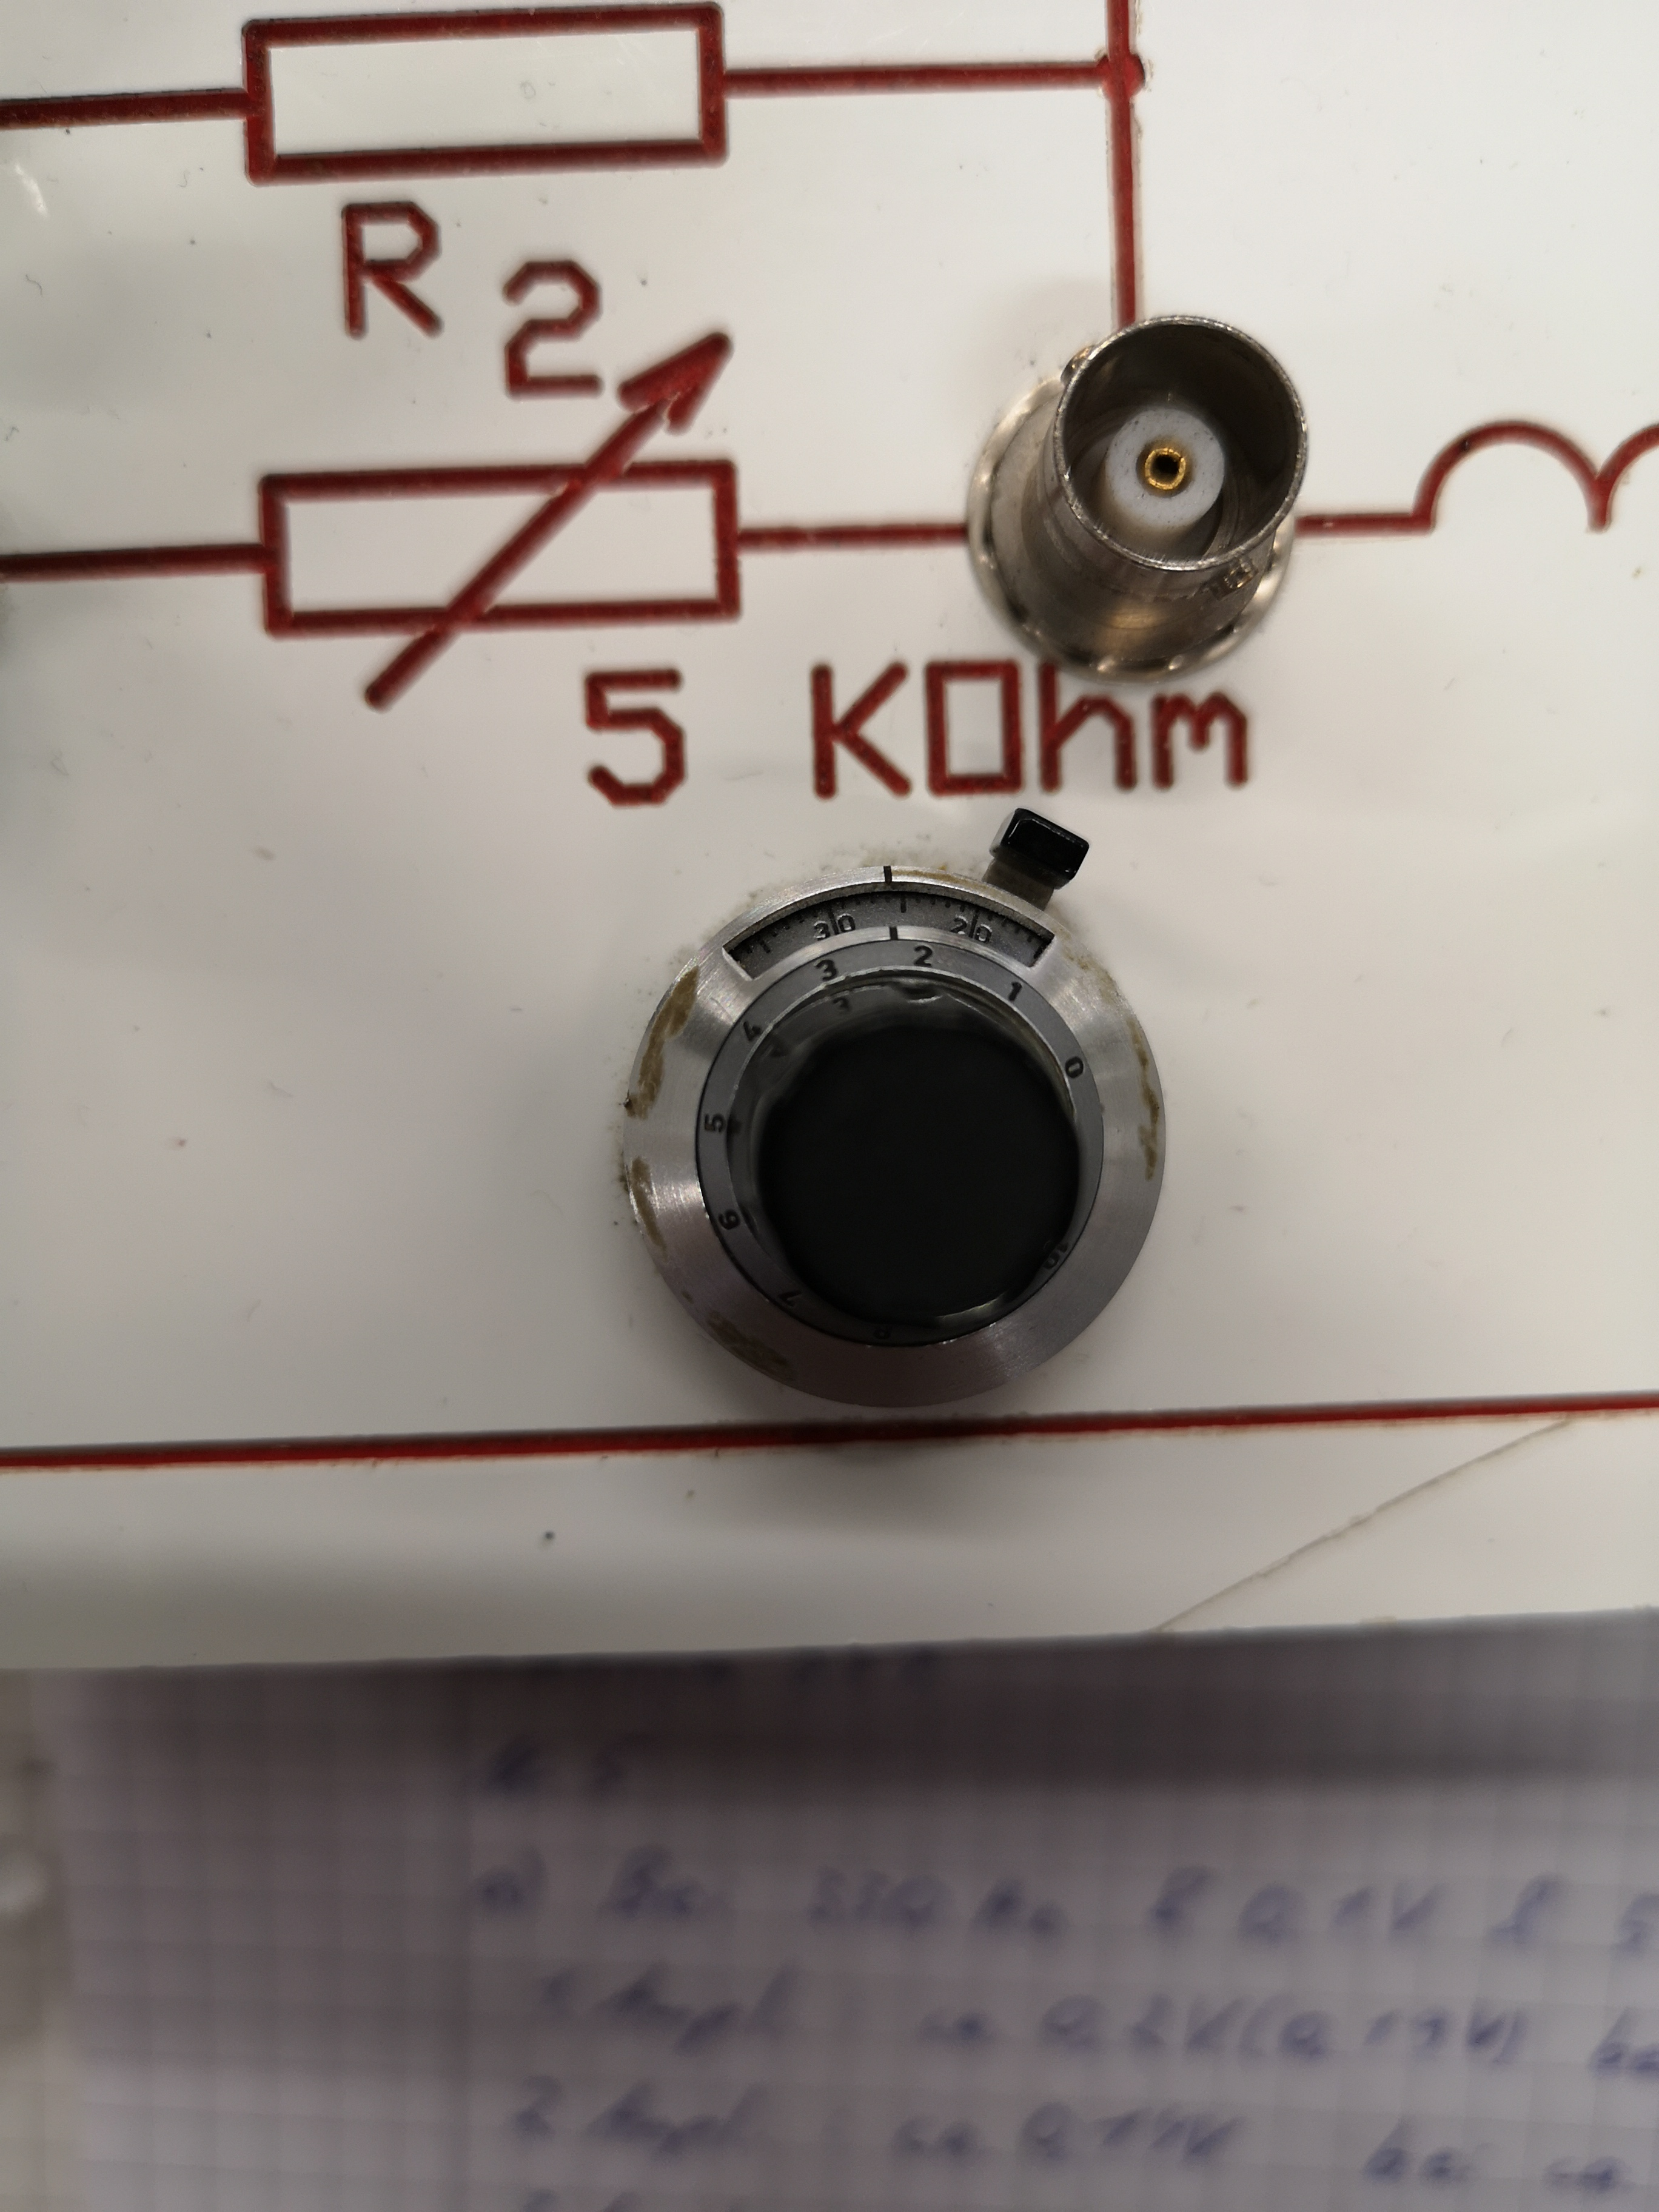
\includegraphics[height=8cm]{content/aperoiode_ohm.jpg}
    \caption{Messung am Drehrad.}
    \label{fig:drehohm}
  \end{subfigure}
  %\caption{Zwei Logos, Abbildung \subref{fig:TU}: Das TU-Logo.}
  %\label{fig:logos}
\end{figure}

Mithilfe eines einfachen Dreisatzes lässt sich dieser Wert auf einen effektiven Dämpfungswiderstand von \(R_{ap}\) = 1,13k\Omega zurückführen.

\begin{table}
  \centering
  \caption{Dreisatz}
  \label{tab:drei}
  \begin{tabular}{c c}
    \midrule
    10 & 5k\(\Omega\)\\
    2.26 & 1.13k\(\Omega\)\\
    \bottomrule
  \end{tabular}
\end{table}
Die Formel für den Widerstand \(R_{ap}\) lautet:
\begin{equation}
  R_{ap} = 2\cdot\sqrt{\frac{L}{C}}
\end{equation}
Mit den gegebenen Werten L = 3.5\pm0.01mH und C = 5.00\pm0.02nF ergibt sich daraus ohne Fehlerrechnung:
\begin{equation}
  R_{ap} = 1673.32\Omega
\end{equation}
Die Diskrepanz liegt bei 543.32\(\Omega\).

\newpage
\subsection{Verhältnis von \(U_C\) zur Frequenz}
Die Kondensatorspannung \(U_C\) nimmt anfangs mit steigender Frequenz ebenfalls zu, bis sie bei ca 35kHz wieder abnimmt.
\begin{table}
  %Messwerte aus c)
  \centering
  \caption{Tabelle der Messwerte mit \(R_2\)}
  \label{tab:tab2}
  \begin{tabular}{c c}
    \toprule
    $\nu$ in $kHz$ & \(U_C\) in $V$\\
    \midrule
    5 & 0.8\\
    10 & 0.85\\
    15 & 0.9\\
    20 & 1\\
    25 & 1.2\\
    30 & 1.6\\
    35 & 2\\
    40 & 1.7\\
    45 & 1.1\\
    50 & 0.75\\
    55 & 0.55\\
    60 & 0.43\\
    65 & 0.34\\
    70 & 0.28\\
    75 & 0.24\\
    \bottomrule
  \end{tabular}
\end{table}

\begin{figure}
  %Plot der Messwerte aus c)
  \centering
  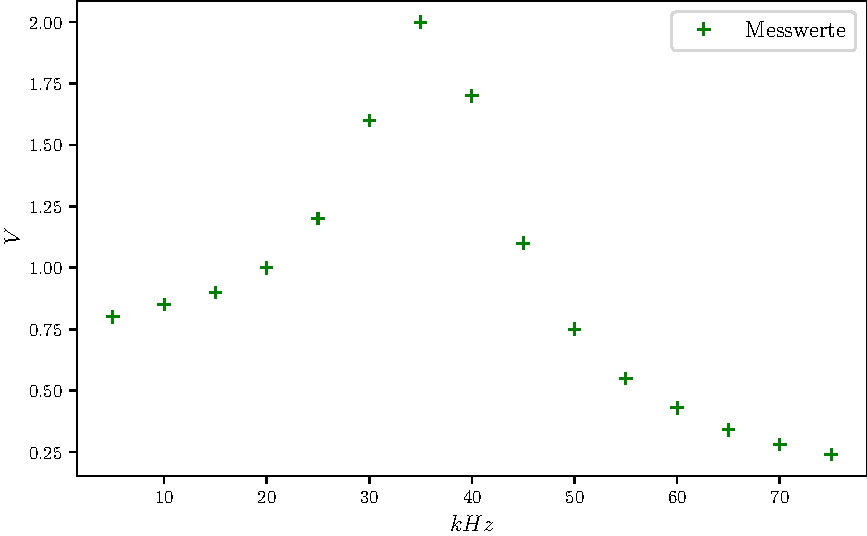
\includegraphics{plot2.pdf}
  \caption{Plot2.}
  \label{fig:plot2}
\end{figure}

\newpage
\subsection{Phasendifferenz vor und nach dem Schwingkreis}
Um den Phasenunterschied zu messen erfordert es die Distanz a zwischen den Signalen auf der x-Achse und die Wellenlänge b.\\

\begin{figure}[htb]
  \centering
  \caption{Formel zu Phasendifferenz.}
  \label{fig:phasenart}
  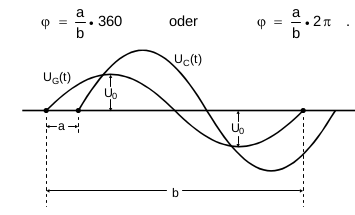
\includegraphics[scale = 0.5]{content/Phasendar.png}
\end{figure}

In \autoref{fig:phasenart} ist der Messvorgang verdeutlicht.\\

\begin{table}[htb]
  %Messwerte aus d)
  \centering
  \caption{Tabelle der Messwerte mit Phasenunterschied.}
  \label{tab:tab3}
  \begin{tabular}{c c c}
    \toprule
    $\nu$ in $kHz$ & a in $\mu$s & b in $\mu$s\\
    \midrule
    140 & 0.08 & 7\\
    120 & 0.1 & 8\\
    100 & 0.2 & 10\\
    80 & 0.3 & 11\\
    60 & 0.8 & 15.5\\
    40 & 4.2 & 22.5\\
    \bottomrule
  \end{tabular}
\end{table}
\newpage
Die \autoref{tab:tab3} enthält die Messdaten vor der Rechnung und \autoref{tab:tab4} zeigt die Korrelation von Frequenz und Phasenverschiebung.\\

\begin{table}[htb]
  %Messwerte aus d) mit Delta Phi
  \centering
  \caption{Tabelle der Messwerte mit \(\Delta\phi\)}
  \label{tab:tab4}
  \begin{tabular}{c c}
    \toprule
    $\nu$ in $kHz$ & $\Delta\phi$ in °\\
    \midrule
    140 & 67.2\\
    120 & 18.58\\
    100 & 9.82\\
    80 & 7.2\\
    60 & 4.5\\
    40 & 4.11\\
    \bottomrule
  \end{tabular}
\end{table}

Die Werte in \autoref{fig:plot3} zeigen einen exponentiellen Abfall bei höherer Frequenz.\\

\begin{figure}[htb]
  %Plot zu Messwerten aus d)
  \centering
  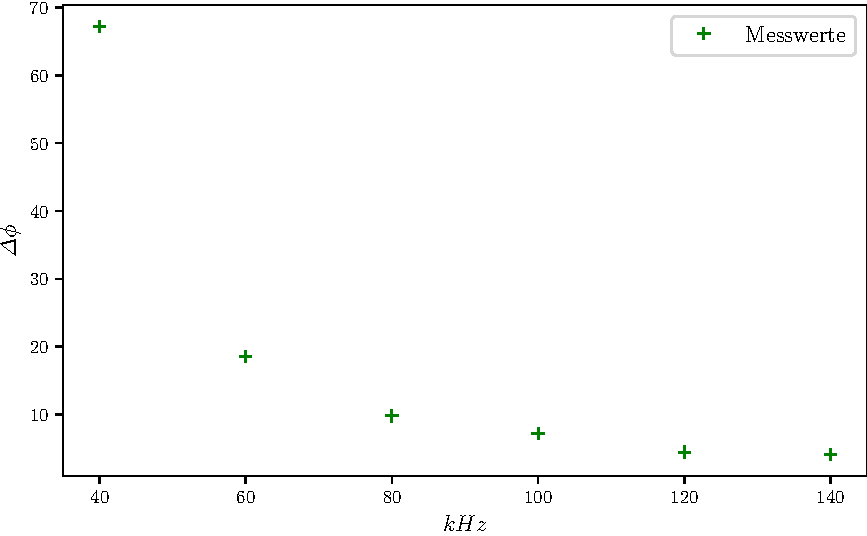
\includegraphics[scale = 0.7]{plot3.pdf}
  \caption{Plot3.}
  \label{fig:plot3}
\end{figure}

%Siehe \autoref{fig:plot}!
